\documentclass[12pt, titlepage]{article}

\usepackage{fullpage}
\usepackage{booktabs}
\usepackage{tabularx}
\usepackage{hyperref}
\usepackage{xcolor}
\hypersetup{
    colorlinks,
    citecolor=black,
    filecolor=black,
    linkcolor=red,
    urlcolor=blue
}
\usepackage{graphicx}
\graphicspath{ {./images/} }
\usepackage{float}
\usepackage[round]{natbib}

%% Comments

\usepackage{color}

\newif\ifcomments\commentstrue %displays comments
%\newif\ifcomments\commentsfalse %so that comments do not display

\ifcomments
\newcommand{\authornote}[3]{\textcolor{#1}{[#3 ---#2]}}
\newcommand{\todo}[1]{\textcolor{red}{[TODO: #1]}}
\else
\newcommand{\authornote}[3]{}
\newcommand{\todo}[1]{}
\fi

\newcommand{\wss}[1]{\authornote{blue}{SS}{#1}} 
\newcommand{\plt}[1]{\authornote{magenta}{TPLT}{#1}} %For explanation of the template
\newcommand{\an}[1]{\authornote{cyan}{Author}{#1}}

%% Common Parts

\newcommand{\progname}{Software Engineering} % PUT YOUR PROGRAM NAME HERE
\newcommand{\authname}{Team 14, Reach
\\ Aamina Hussain
\\ David Moroniti
\\ Anika Peer
\\ Deep Raj
\\ Alan Scott} % AUTHOR NAMES                  

\usepackage{hyperref}
    \hypersetup{colorlinks=true, linkcolor=blue, citecolor=blue, filecolor=blue,
                urlcolor=blue, unicode=false}
    \urlstyle{same}
                                


\begin{document}

\title{Verification and Validation Report: \progname}
\author{\authname}
\date{\today}

\maketitle

\pagenumbering{roman}

\section{Revision History}

\begin{tabularx}{\textwidth}{p{3cm}p{2cm}X}
  \toprule {\bf Date} & {\bf Version} & {\bf Notes}                              \\
  \midrule
  03/04/2024          & 1.0           & Add results for some functional tests    \\
  03/06/2024          & 1.1           & Add results for unit tests + reflection  \\
  03/06/2024          & 1.0           & Add results for some nonfunctional tests \\
  \bottomrule
\end{tabularx}

~\newpage

\section{Symbols, Abbreviations and Acronyms}

\renewcommand{\arraystretch}{1.2}
\begin{tabular}{l l}
  \toprule
  \textbf{symbol} & \textbf{description} \\
  \midrule
  T               & Test                 \\
  UNT             & Unit Test            \\
  UT              & Usability Test       \\
  ST              & Searching Test       \\
  DT              & Data Test            \\
  BT              & Bookmarking Test     \\
  PIT             & Program Info Test    \\
  PT              & Performance Test     \\
  \bottomrule
\end{tabular}\\


\newpage

\tableofcontents

\listoftables %if appropriate

\listoffigures %if appropriate

\newpage

\pagenumbering{arabic}

\section{Functional Requirements Evaluation}

\noindent\large{\textbf{Authentication}}

\normalsize

\begin{enumerate}
  \item AT-1
        Result: \textcolor{green}{Passed} - The tester was able to successfully create an account, and was redirected to the next page,
        indicating that the account was created successfully. Therefore, this test was successful.
  \item AT-2
        Result: \textcolor{green}{Passed} - The tester was not able to create an account with an email that was already in use,
        and was blocked from clicking the register button. Therefore, this test was successful.
  \item AT-3
        Result: \textcolor{green}{Passed} - The tester was not able to create an account with a password that did not meet the NIST guidelines.
        Therefore, this test passed.
  \item AT-4
        Result: \textcolor{green}{Passed} - The tester was able to successfully log in, the user was redirected to the home page,
        indicating that the login was successful. Therefore, this test was successful.
  \item AT-5
        Result: \textcolor{green}{Passed} - The tester was not able to log in with a username that did not exist, an error message was displayed,
        and the user was not able to proceed to the next page. Therefore, this test was successful.
  \item AT-6
        Result: \textcolor{gray}{Not run} - Feature being tested was not yet implemented at the time of testing.
  \item AT-7
        Result: \textcolor{gray}{Not run} - Feature being tested was not yet implemented at the time of testing.
  \item AT-8
        Result: \textcolor{green}{Passed} - The tester was able to successfully log out, and was redirected to the login page.
        Therefore, this test was successful.
\end{enumerate}

\noindent\large{\textbf{User Data}}

\normalsize

\begin{enumerate}
  \item DT-1
        Result: \textcolor{green}{Passed} - New account can successfully be created, and data is stored successfully in the database. Therefore, the tester was able to verify that the data is
        persistent, and so this test was successful.
  \item DT-2
        Result: \textcolor{green}{Passed} - Account information can successfully be updated, and the changes are reflected in the database. Therefore, the tester was able to verify
        that the updates are persistent, and so this test was successful.
  \item DT-3
        Result: \textcolor{gray}{Not run} - reason being that the database application we used will ensure the issue brought up by this test can never happen.\\
\end{enumerate}

\noindent\large{\textbf{Email}}

\normalsize

\begin{enumerate}
  \item ET-1
        Result: \textcolor{gray}{Not Run} - This feature implementation was not complete at the time of testing, and so the test was not conducted.
\end{enumerate}

\noindent{\large{\textbf{Program Information}}}

\normalsize

\begin{enumerate}
  \item PIT-1 \textcolor{green}{Passed} - The tester was able to verify that the FAQ system can be viewed by a user (whether they are logged in or not), and so this test was successful.\\
\end{enumerate}

\noindent{\large{\textbf{Searching}}}

\normalsize

\begin{enumerate}
  \item ST-1 \textcolor{gray}{Not run} - Functionality tested by this test was removed from the requirements prior to conducting testing.
  \item ST-2 \textcolor{green}{Passed} - The tester was able to conduct a search based on a patient profile, and view the resulting trials. Therefore, this test was
        successful.
  \item ST-3 \textcolor{red}{Failed} - When attempting to search for trials with no profile data selected, the app did not behave as intended (it
        still tried to conduct a search), therefore this test was unsuccessful.
  \item ST-4 \textcolor{green}{Passed} - The tester was able to switch between multiple profiles, and conduct a search based on each respective profile.
  \item ST-5 \textcolor{green}{Passed} - Upon selecting a displayed trial, the tester was able to verify that the location displayed on the map updates and displays correctly.\\

\end{enumerate}

\noindent{\large{\textbf{Bookmarking}}}

\normalsize

\begin{enumerate}
  \item BT-1 \textcolor{green}{Passed} - The tester was able to save a trial, and view the trial in the bookmarks page. Additionally, there was an indication that
        the trial was saved, upon saving the trial. Therefore, this test was successful.
  \item BT-2 \textcolor{green}{Passed} - The tester was able to delete a trial that was previously saved, and verified that the deletion was recognized in the frontned (i.e., by
        no longer being part of the list of saved trials). Therefore, this test was successful.
  \item BT-3 \textcolor{green}{Passed} - The tester was able to verify that the details provided by the saved trial are the same as the details related to the trial
        on the search trial page.
  \item BT-4 \textcolor{green}{Passed} - The tester was able to verify that the saved trials are filtered correctly upon selecting a profile to filter by. When selecting a
        profile, only the trials saved under that profile are displayed, and when selecting no profile, all saved trials are displayed to the user.

\end{enumerate}


\section{Nonfunctional Requirements Evaluation}

\subsection{Usability}

In order to test usability, we created and conducted a Usability Test \& Survey (in section 6.2 of the
\href{https://github.com/davimang/REACH/blob/main/docs/VnVPlan/VnVPlan.pdf}{VnVPlan}) with five different participants.
The results of this test can be found in \href{https://github.com/davimang/REACH/blob/main/docs/VnVReport/UsabilityTestResults/UsabilityTestResults.pdf}{Usability Test Results}.
The following tests were conducted as part of the usability test:

\begin{enumerate}
  \item UT-1 \textcolor{green}{Passed} - On average, the usability test participants rated their ease to complete this test (navigating to the sign in page) a 4.6 on average. As this is above the minimum rating of 3.5, the test passes.
  \item UT-2 \textcolor{green}{Passed} - On average, the usability test participants rated their ease to complete this test (navigating to the registration page) a 4.8 on average. As this is above the minimum rating of 3.5, the test passes.
  \item UT-3 \textcolor{green}{Passed} - On average, the usability test participants rated their ease to complete this test (registering a new account) a 4.2 on average. As this is above the minimum rating of 3.5, the test passes.
  \item UT-4 \textcolor{green}{Passed} - On average, the usability test participants rated their ease to complete this test (searching for clinical trials) a 3.6 on average. As this is above the minimum rating of 3.5, the test passes.
  \item UT-5 \textcolor{green}{Passed} - On average, the usability test participants rated their ease to complete this test (viewing more details of a trial) a 3.6 on average. As this is above the minimum rating of 3.5, the test passes.
  \item UT-6 \textcolor{green}{Passed} - On average, the usability test participants rated their ease to complete this test (bookmarking a trial) a 4.4 on average. As this is above the minimum rating of 3.5, the test passes.
  \item UT-7 \textcolor{green}{Passed} - On average, the usability test participants rated their ease to complete this test (viewing bookmarked trials) a 3.8 on average. As this is above the minimum rating of 3.5, the test passes.
  \item UT-8 \textcolor{red}{Failed} - On average, the usability test participants rated their ease to complete this test (navigating to the search trials page) a 2.4 on average. As this is below the minimum rating of 3.5, the test fails. According to feedback we received when conducting the Usability Test \& Survey, participants felt there was no clear way to navigate to the Search Trials page and thus gave this test a low rating.
  \item UT-9 \textcolor{green}{Passed} - On average, the usability test participants rated their ease to complete this test (viewing account information) a 5 on average. As this is above the minimum rating of 3.5, the test passes.
  \item UT-10 \textcolor{green}{Passed} - On average, the usability test participants rated their ease to complete this test (adding a new profile) a 4.8 on average. As this is above the minimum rating of 3.5, the test passes.
  \item UT-11 \textcolor{green}{Passed} - On average, the usability test participants rated their ease to complete this test (navigating to the REACH home page) a 5 on average. As this is above the minimum rating of 3.5, the test passes.
  \item UT-12 \textcolor{green}{Passed} - On average, 100\% of users did not report any issues navigating the interface after changing their preferred language. As this is above the minimum 95\% of users, the test passes.
\end{enumerate}

\noindent The following graph summarizes and displays the results of the usability test (visualizing the passed/failed tests UT-1 to UT-11):

\begin{figure}[H]
  \centering
  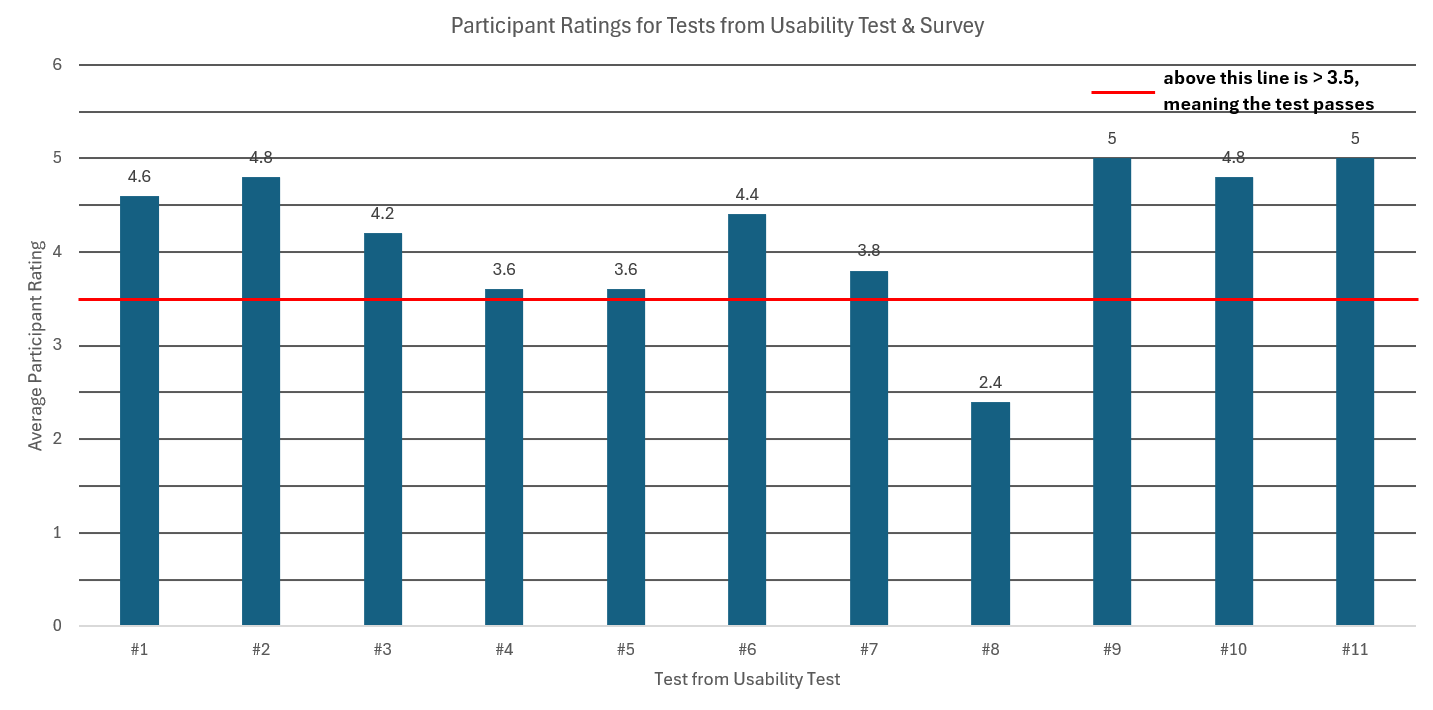
\includegraphics[width=1\linewidth]{images/AverageRatingsUT.png}
  \caption{Average Participants Ratings for Tests in Usability Test}
  \label{fig:figure1}
\end{figure}

\subsection{Performance}
\begin{enumerate}
  \item PT-1 \textcolor{green}{Passed} - On average, the tests to load trials take on average 4.1 seconds. As this is below the benchmark of 5 seconds, the test passes.
  \item PT-2 \textcolor{green}{Passed} - All endpoints were tested manually to measure the time taken to establish connections between endpoints. All tests succeeded in under 1 second, so the tests pass.
\end{enumerate}

\subsection{Maintainability}
\begin{enumerate}
  \item MT-1 \textcolor{red}{Failed} - Modified code in the pull request has been routinely and automatically linted by a Github CI component upon creation of pull requests. Some pull requests have been rejected by the linter, so the test fails.
\end{enumerate}

\subsection{Security}
\begin{enumerate}
  \item OT-1 \textcolor{gray}{Not run} - Application was updated to display a fixed amount (5) of results at a time. As the application no longer needs to display all available trials, this test is no longer necessary.
  \item OT-2 \textcolor{green}{Passed} - Several testers accessed the web application from their respective devices and tried out the main functions of the application. All testers consistently rated the performance above 7, so the test passed.
\end{enumerate}

\subsection{Operational and Environmental}
\begin{enumerate}
  \item SEC-1 \textcolor{green}{Passed} - The tester entered the password "pass" which does not conform to the NIST guidelines. The password was not accepted and the account was not created, so the test passes.
  \item SEC-2 \textcolor{green}{Passed} - Two tests were run. Firstly, a tester with the correct password but incorrect username attempted to access the database. This test was successful as the tester was denied access to the database. Secondly, a tester with correct credentials attempted to log into the database. This attempt was successful, so the second part of the test was also successful.
\end{enumerate}

\subsection{Legal}
\begin{enumerate}
  \item SEC-1 \textcolor{gray}{Not run} - This test case has not been run as the user consent function has not been implemented.
\end{enumerate}


\section{Comparison to Existing Implementation}

This section will not be appropriate for every project.

\section{Unit Testing}

\begin{enumerate}
  \item UNT-1
        Result: \textcolor{green}{Passing}
  \item UNT-2
        Result: \textcolor{green}{Passing}
  \item UNT-3
        Result: \textcolor{green}{Passing}
  \item UNT-4
        Result: \textcolor{green}{Passing}
  \item UNT-5
        Result: \textcolor{green}{Passing}
  \item UNT-6
        Result: \textcolor{green}{Passing}
  \item UNT-7
        Result: \textcolor{green}{Passing}
  \item UNT-8
        Result: \textcolor{green}{Passing}
  \item UNT-9
        Result: \textcolor{red}{Failing} - Functionality that is tested by this unit test is currently under a slight rework, which is causing the test to fail.
  \item UNT-10
        Result: \textcolor{red}{Failing} - Functionality that is tested by this unit test is currently under a slight rework which is causing the test to fail.
  \item UNT-11
        Result: \textcolor{green}{Passing}
  \item UNT-12
        Result: \textcolor{green}{Passing}
  \item UNT-13
        Result: \textcolor{green}{Passing}
  \item UNT-14
        Result: \textcolor{green}{Passing}
  \item UNT-15
        Result: \textcolor{green}{Passing}
  \item UNT-16
        Result: \textcolor{green}{Passing}
  \item UNT-17
        Result: \textcolor{green}{Passing}
  \item UNT-18
        Result: \textcolor{green}{Passing}
  \item UNT-19
        Result: \textcolor{green}{Passing}
  \item UNT-20
        Result: \textcolor{green}{Passing}
  \item UNT-21
        Result: \textcolor{green}{Passing}
\end{enumerate}

\section{Changes Due to Testing}

In terms of receiving feedback on our designs, our team has cultivated a diverse group of potential users
in order ascertain that our design is meeting the requirements of the primary stakeholders.
More specifically, throughout the term,
we held biweekly focus meetings with our supervisors, Dr. Ho and Dr. Scallan, where we received crucial
pointers regarding key design issues in visibility, consistency and clarity. \newline

A major component of our design, the map feature for displaying trial locations,
was not seriously considered until we received feedback from our supervisors. They impressed upon
us the importance of having the feature fully functional early on in the development process.
We thought this was the case after revision 0 and had tested that it was displaying locations
accurately. However, we did not account for the resilience of the program and found that every few reloads
the map might not show any results for trials. This was a major design issue
especially because the majority of the trials had associated locations and as such this could not be
attributed to anything but the way we embedded the map.
By unit testing this and gaining an understanding of the functionality at a granular level,
we were able to ensure that the map displayed every time. \newline

Another piece of feedback that helped us in the development process
had to do with limiting distances for trial searches. Prior to this feedback,
we did not have a limit on how far away a trial could be. This potentially linked
users to trials that could be over 500 km away from their main address. This issue did not
cost us too much in terms of usability metrics (it was not a big factor) but by changing it
we improved user experience significantly as trial results were more relevant to users. \newline

Additionally, as we have more users test the application, we plan to continue making incremental changes
to the platform that will center on UI/UX improvements from a front-end lens.


\section{Automated Testing}
Using pipelines, we streamlined our testing process via the integration of unit
testing into our linter workflow. Before merging our code into the main branch, we adhere
to running multistage pipelines that lint and use use pytest to test our code.
Pytest serves as our testing framework
due to its robust nature and automation capabilities. The key functionality we tested includes (but is not limited to):
filters, saving trials, profile creation, and age and distance calculations. Pytest, having a high degree of organization and flexibility
in terms of execution, is perfect
for our particular use case. It simplifies the process of running multiple tests and interpreting results
allowing for better collaboration and clarity between team members.


\section{Trace to Requirements}

For test case to requirement traceability, see section 4.3 in the \href{https://github.com/davimang/REACH/blob/main/docs/VnVPlan/VnVPlan.pdf}{VnVPlan}.
\section{Trace to Modules}
For test case to module traceability, see section 5.3 in the \href{https://github.com/davimang/REACH/blob/main/docs/VnVPlan/VnVPlan.pdf}{VnVPlan}.

\section{Code Coverage Metrics}

As this project consists mainly of using external APIs and libraries, we decided it was not necessary
for us to test our code using any code coverage software. Our backend code mainly consists of different
models to represent and store our data in the database, as well as communication with the clinicaltrials.gov APIs.
Our frontend code similarly just displays data fetched from the relevant APIs. This indicates that testing for code
coverage would not be beneficial in our case.

\bibliographystyle{plainnat}
%\bibliography{../../refs/References}

\newpage{}
\section*{Appendix --- Reflection}

The information in this section will be used to evaluate the team members on the
graduate attribute of Reflection.  Please answer the following question:

\begin{enumerate}
  \item In what ways was the Verification and Validation (VnV) Plan different
        from the activities that were actually conducted for VnV?  If there were
        differences, what changes required the modification in the plan?  Why did
        these changes occur?  Would you be able to anticipate these changes in future
        projects?  If there weren't any differences, how was your team able to clearly
        predict a feasible amount of effort and the right tasks needed to build the
        evidence that demonstrates the required quality?  (It is expected that most
        teams will have had to deviate from their original VnV Plan.)
\end{enumerate}

There were a few ways in which the VnV plan was different from the activities that were actually conducted. First, there were a few tests written
for functionality that is no longer planned to be in the app. For example, the email notification system/module is no longer in scope, and as a result,
tests were obviously not conducted for this module. Furthermore, there were some tests that did not need to be done as a direct result of the
implementation, and more specifically, some of the tools that were used in the implementation. For example, a good chunk of the authentication tests did
not actually need to be done, since Django provides an out of the box solution to authenticating users (which we were able to take advantage of). It would be
very difficult to anticipate all of these changes in a future project, since there are so many variables affecting the testing stage (i.e., change in scope,
implementation details, etc..). Fortunately, this is why we follow the iterative process, since it allows us to make continuous updates to our documentation,
ensuring there is always consistency between the plan, report, the app itself, and the other documents (such as SRS, MIS, etc..).


\end{document}